\documentclass{beamer}

\usepackage{multimedia}
\usefonttheme{serif}

\setbeamertemplate{footline}[frame number]{}
\setbeamertemplate{navigation symbols}{}

\usecolortheme{default}
\setbeamercolor{block title}{bg=lily!20,fg=black}
\setbeamercolor{block body}{bg = blue!10, fg = black}
\setbeamertemplate{itemize item}[square]
\setbeamercolor{itemize item}{fg = cyan}
\setbeamercolor{enumerate item}{fg = cyan}

\usetheme{default}

%\setbeamercolor{titlelike}{fg=black}
%Information to be included in the title page:
\title{Sample title}
\author{Anonymous}
\institute{Overleaf}
\date{2021}

\title[About Beamer] %optional
{Pockels effect}

%\subtitle{A short story}

\author[Arthur, Doe] % (optional, for multiple authors)
{A.~Simankovich }

\institute[VFU] % (optional)
{
	Moscow Institute of Physics and Technology
}

\date[VLC 2023] % (optional)
%{Very Large Conference, April 2021}

%\logo{\includegraphics[height=1cm]{overleaf-logo}}

\begin{document}
	
	\frame{\titlepage}
	
	\begin{frame}
		\frametitle{Abstract}
		
		Article studies birefringence and Pockels effect on $\text{LiNbO}_3$ crystal. Theoretical description of effects provided. Interference patterns are examined. Difference of refractive indices $n_e - n_o$ is estimated numerically. Pockels effect is observed. Characteristic values of $U_{\lambda/2}$, $E_{\lambda/2}$ are evaluated.
	\end{frame}
	
	\begin{frame}
		\frametitle{Birefringence}
		%\vspace{-30pt}
		In materials refractive index can depend on the polarization and direction of light propagation.
		\begin{figure}
			\footnotesize
			\centering
			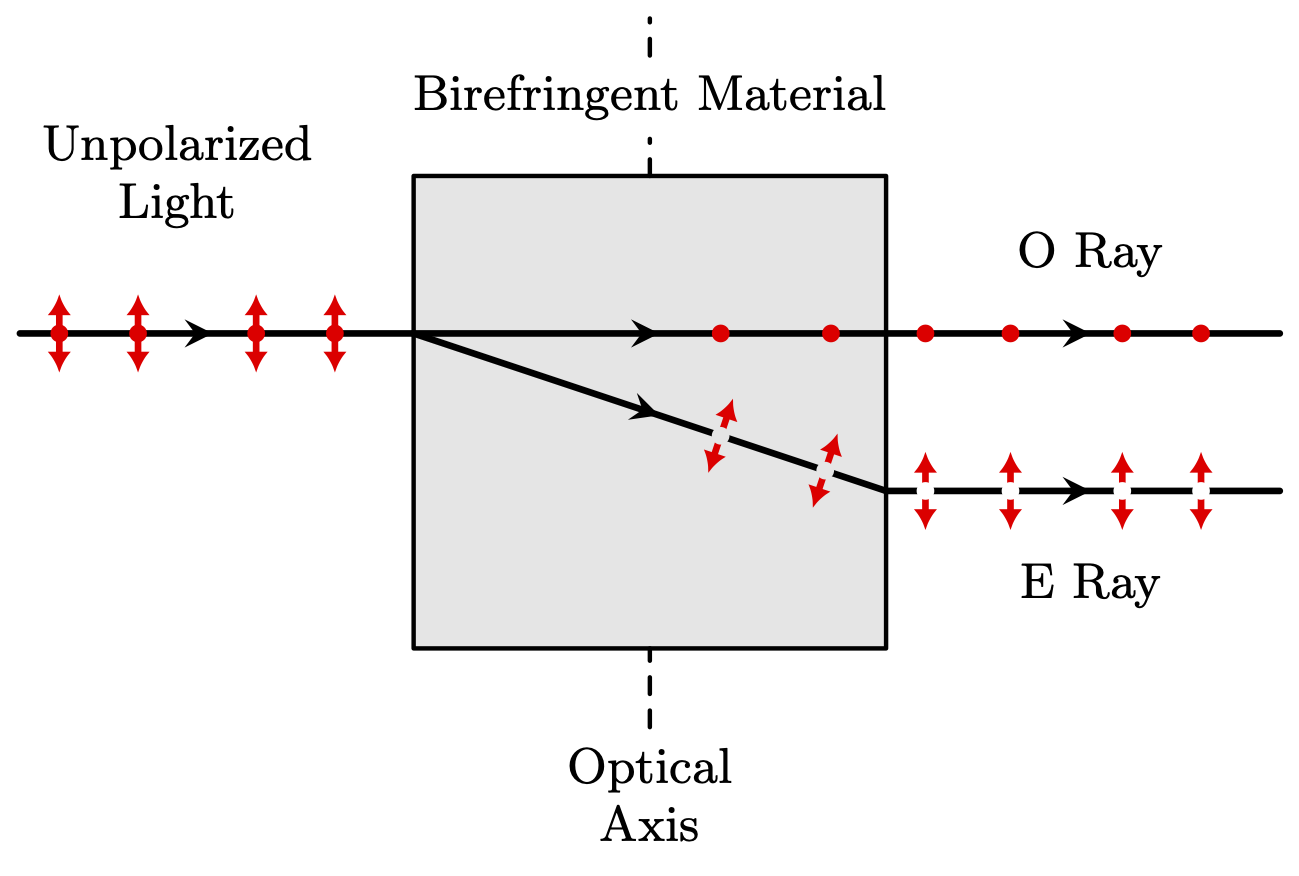
\includegraphics[width=\linewidth]{res/birefringence}
			\vspace{-5pt}
			\footnotesize
			\caption{\footnotesize Ordinary ($n_o$) and extraordinary ($n_e$) waves scheme.}
		\end{figure}		
	\end{frame}


	\begin{frame}
		\frametitle{Scatter plate}		
		\begin{figure}
			\footnotesize
			\centering
			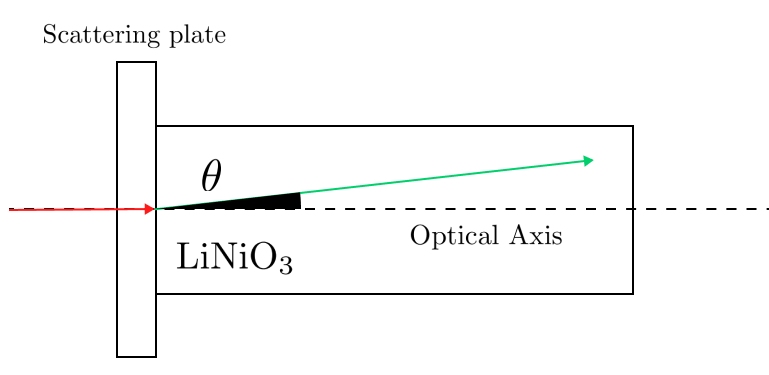
\includegraphics[width=0.9\linewidth]{res/theta_propagation}
			\vspace{-5pt}
			\footnotesize
			\caption{\footnotesize Ray propogation}
		\end{figure}
		
		For ordinary wave $n$ stays the same: $n_o(\theta) = n_o$.
		
		Extraordinary wave:
		\footnotesize
		$$\frac{1}{n_e^2(\theta)} = \frac{\cos^2{\theta}}{n_o^2} + \frac{\sin^2{\theta}}{n_e^2} \implies n_e^2(\theta) \approx n_o - (n_o - n_e) \theta^2.$$
		
	\end{frame}	
			
	\begin{frame}
		\frametitle{Interference observation}
		
		\begin{figure}
			\centering
			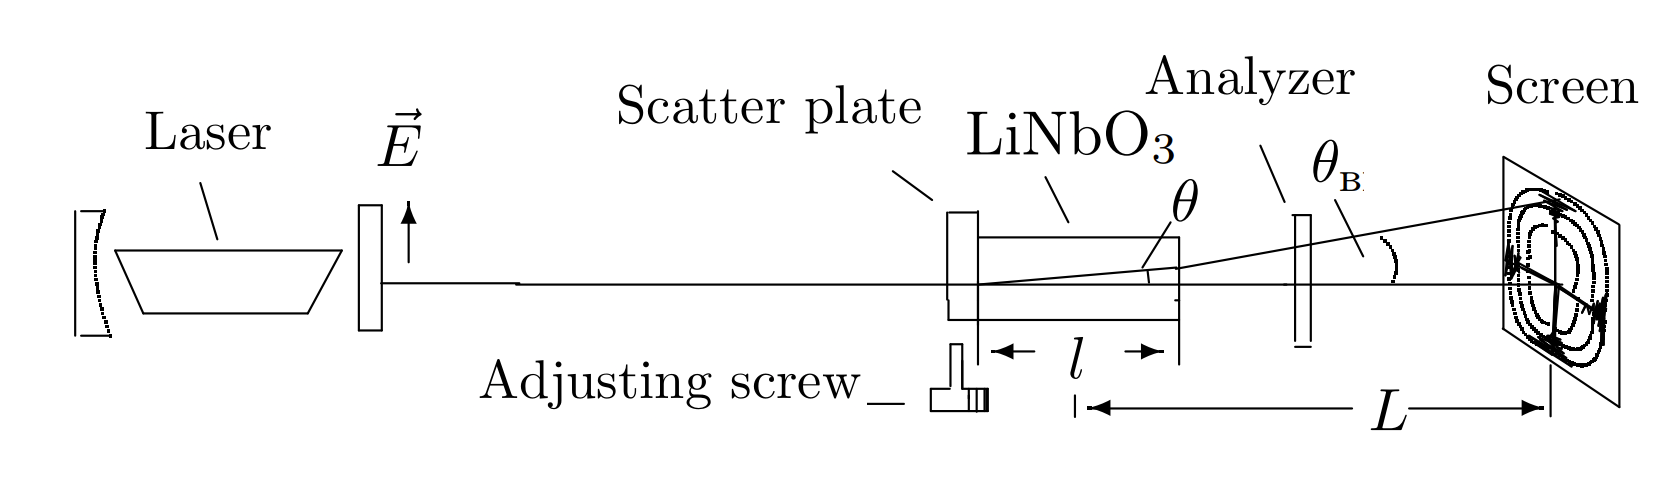
\includegraphics[width=1\linewidth]{res/scheme}
			\caption{Experimental setup}
		\end{figure}
		
		Phase shift between ordinary and extraordinary waves can be estimated:
		$$
		\Delta \varphi = \frac{2\pi}{\lambda}l(n_o - n_e)\theta^2,
		$$
		where $\lambda$ -- wavelength, $l$ -- LiNbO$_3$ crystal length.
	\end{frame}

	\begin{frame}
		\frametitle{Application of analyzer}
		
		\begin{figure}
			\centering
			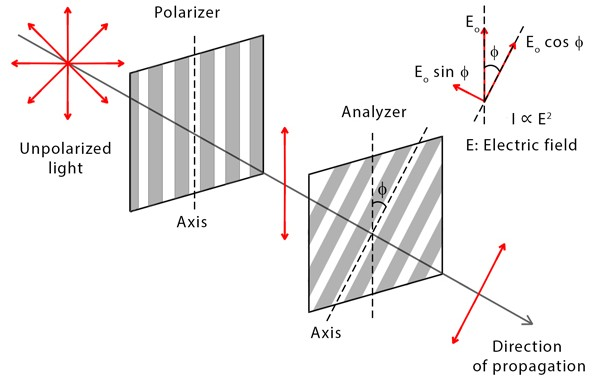
\includegraphics[width=0.8\linewidth]{res/malus_law.jpg}
			\caption{System of analyzer and polarizer}
		\end{figure}
		
		Using analyzer we can project differently polarized light on required axis.
	\end{frame}
	

	\begin{frame}
		\frametitle{Conoscopic interference patterns}
		
		\begin{figure}
			\centering
			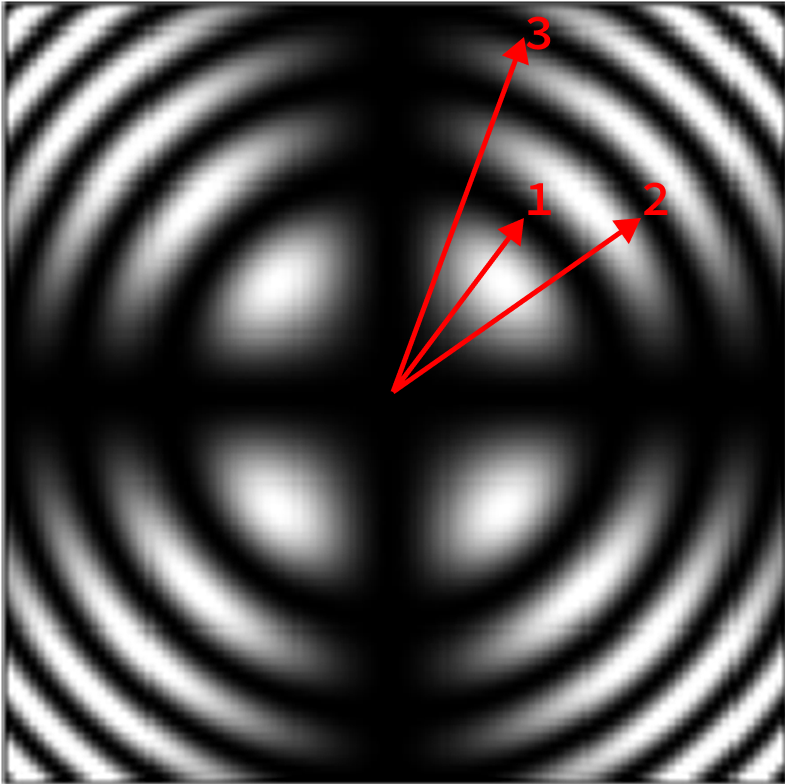
\includegraphics[width=0.5\linewidth]{res/pattern.png}
			\caption{Conoscopic interference pattern with the dark "maltese cross"}
		\end{figure}
		
		\footnotesize
		The radius of the nth ring can be calculated by equating: $\Delta \varphi = 2 \pi m$
		$$r^2_m = \frac{\lambda}{l} \frac{(n_o L)^2}{(n_o - n_e)} m,\;\; m = 1,2...,$$
		
		where $L$ -- distance from crystal to the screen.
	\end{frame}
		
	\begin{frame}
		\frametitle{Pockels effect}
		
		\begin{columns}
			\begin{column}{0.5\linewidth}
				Applying voltage to crystal of LiNbO$_3$ converts it from uniaxial to biaxial.
				Biaxial crystal has 'fast' ($n_0 - \Delta n$) and 'slow' ($n_0 + \Delta n$) axes.
				
			\end{column}
		
			\begin{column}{0.5\linewidth}
				\begin{figure}
					\centering
					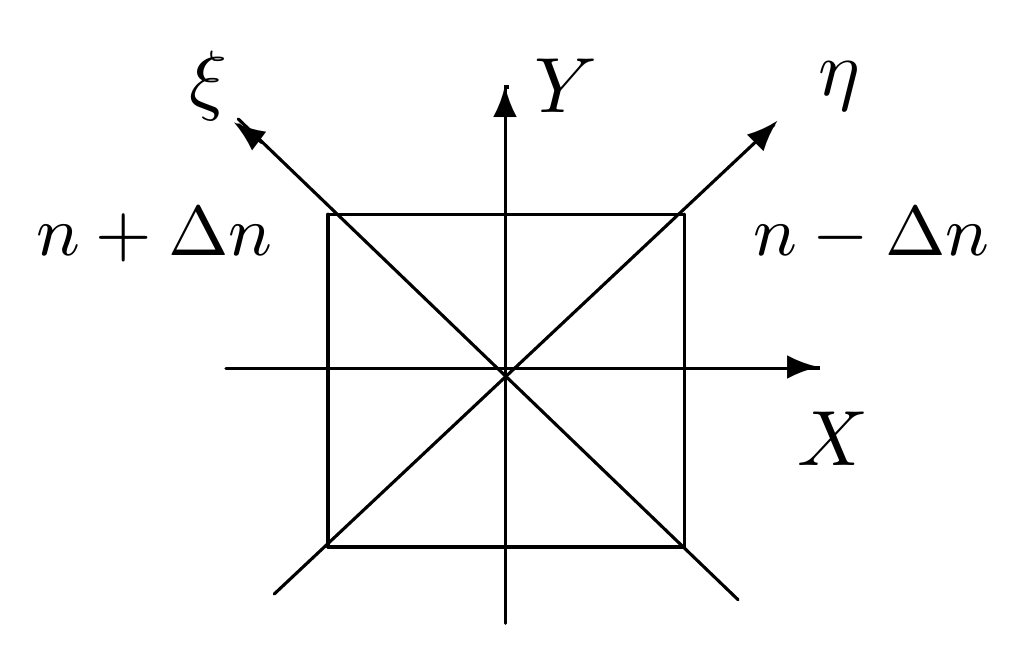
\includegraphics[width=\linewidth]{res/pockels.png}
					\caption{Biaxial structure of crystal}
				\end{figure}
				
			\end{column}
			
		\end{columns}
		\footnotesize
		Phase shift of $E_{\xi}$ and $E_{\eta}$:
		$$ \Delta \varphi = \frac{4\pi}{\lambda} \frac{l}{d} AU,$$
		where $l, \; d$ -- crystal length, width, $A$ -- constant for crystal.
		Decomposing light electric field to $E_{\xi}$ and $E_{\eta}$, evaluating phase shift and projecting on $X$-axis we get:
		$$ E_{\text{out}} = E_0 e^{\omega t - k l} \sin\left(\frac{\Delta \varphi}{2}\right) \qquad I_{\text{out}} = I_0 \sin^2\left(\frac{\pi}{2}\frac{U}{U_{\lambda/2}}\right).$$
	\end{frame}
		
	\begin{frame}[plain,c]	
		\begin{center}
			\huge \usebeamercolor[fg]{frametitle} Measurements and Results
		\end{center}
	\end{frame}	
	
	\begin{frame}
		\frametitle{Experimental Setup}
		
		\begin{figure}
			\centering
			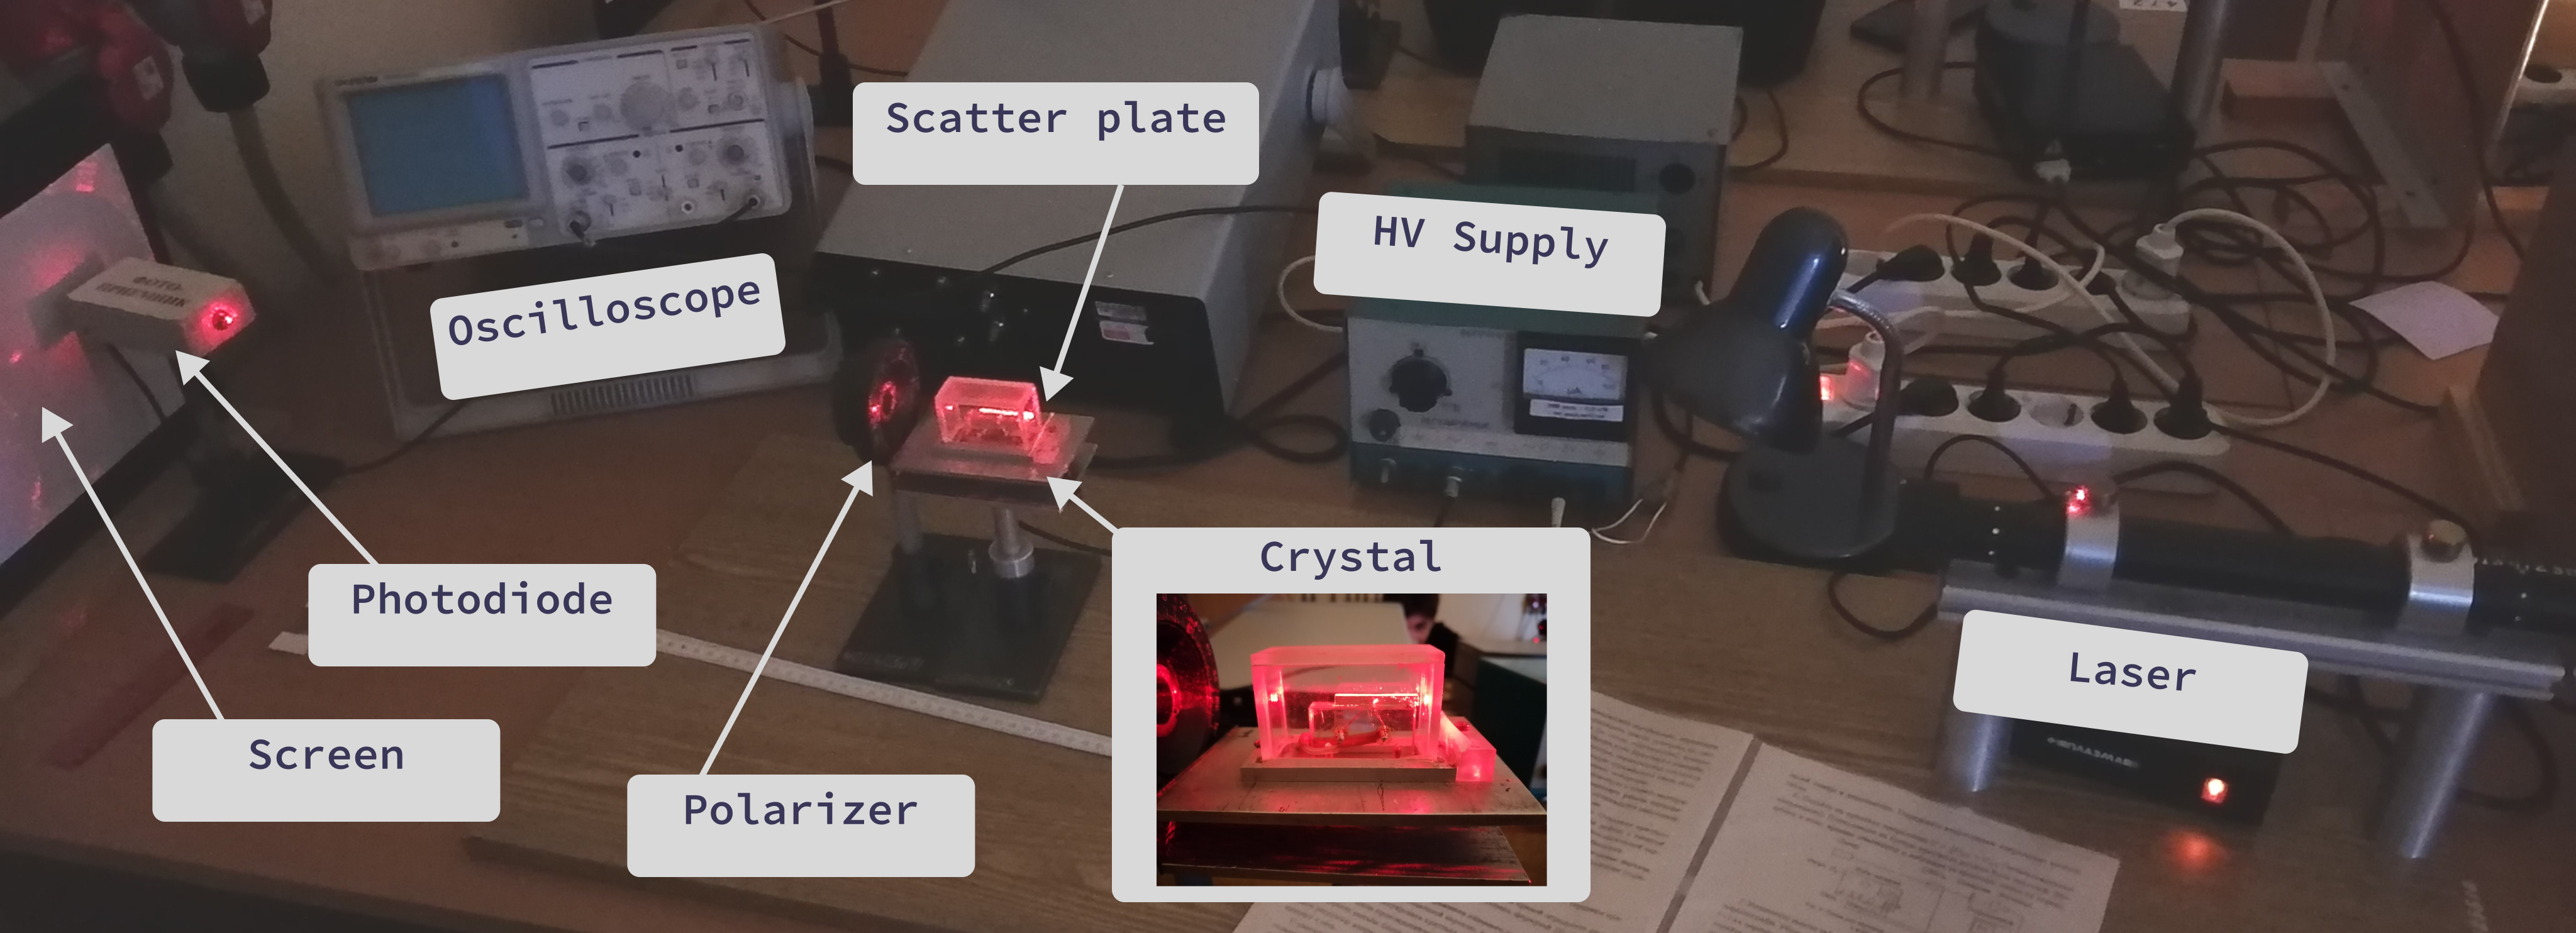
\includegraphics[width=1.0\linewidth]{res/setup1.png}
			\caption{Photo of experimental setup}
		\end{figure}
	
	\begin{itemize}
		\item Crystal dimensions: $3 \; \text{mm} \times 3 \; \text{mm} \times 26 \; \text{mm}$.
		\item Laser wavelength $\lambda = 630$ nm.
		\item HV Supply range: $0 - 1.5$ kV.
		\item Distance between crystal and screen $L = 72$ cm.
	\end{itemize}
		
				
	\end{frame}

	\begin{frame}
		\frametitle{Interference Patterns}
		
		\begin{columns}[t]
			\begin{column}{0.5\textwidth}
				\begin{figure}
					\vspace{-20pt}
					
					\centering
					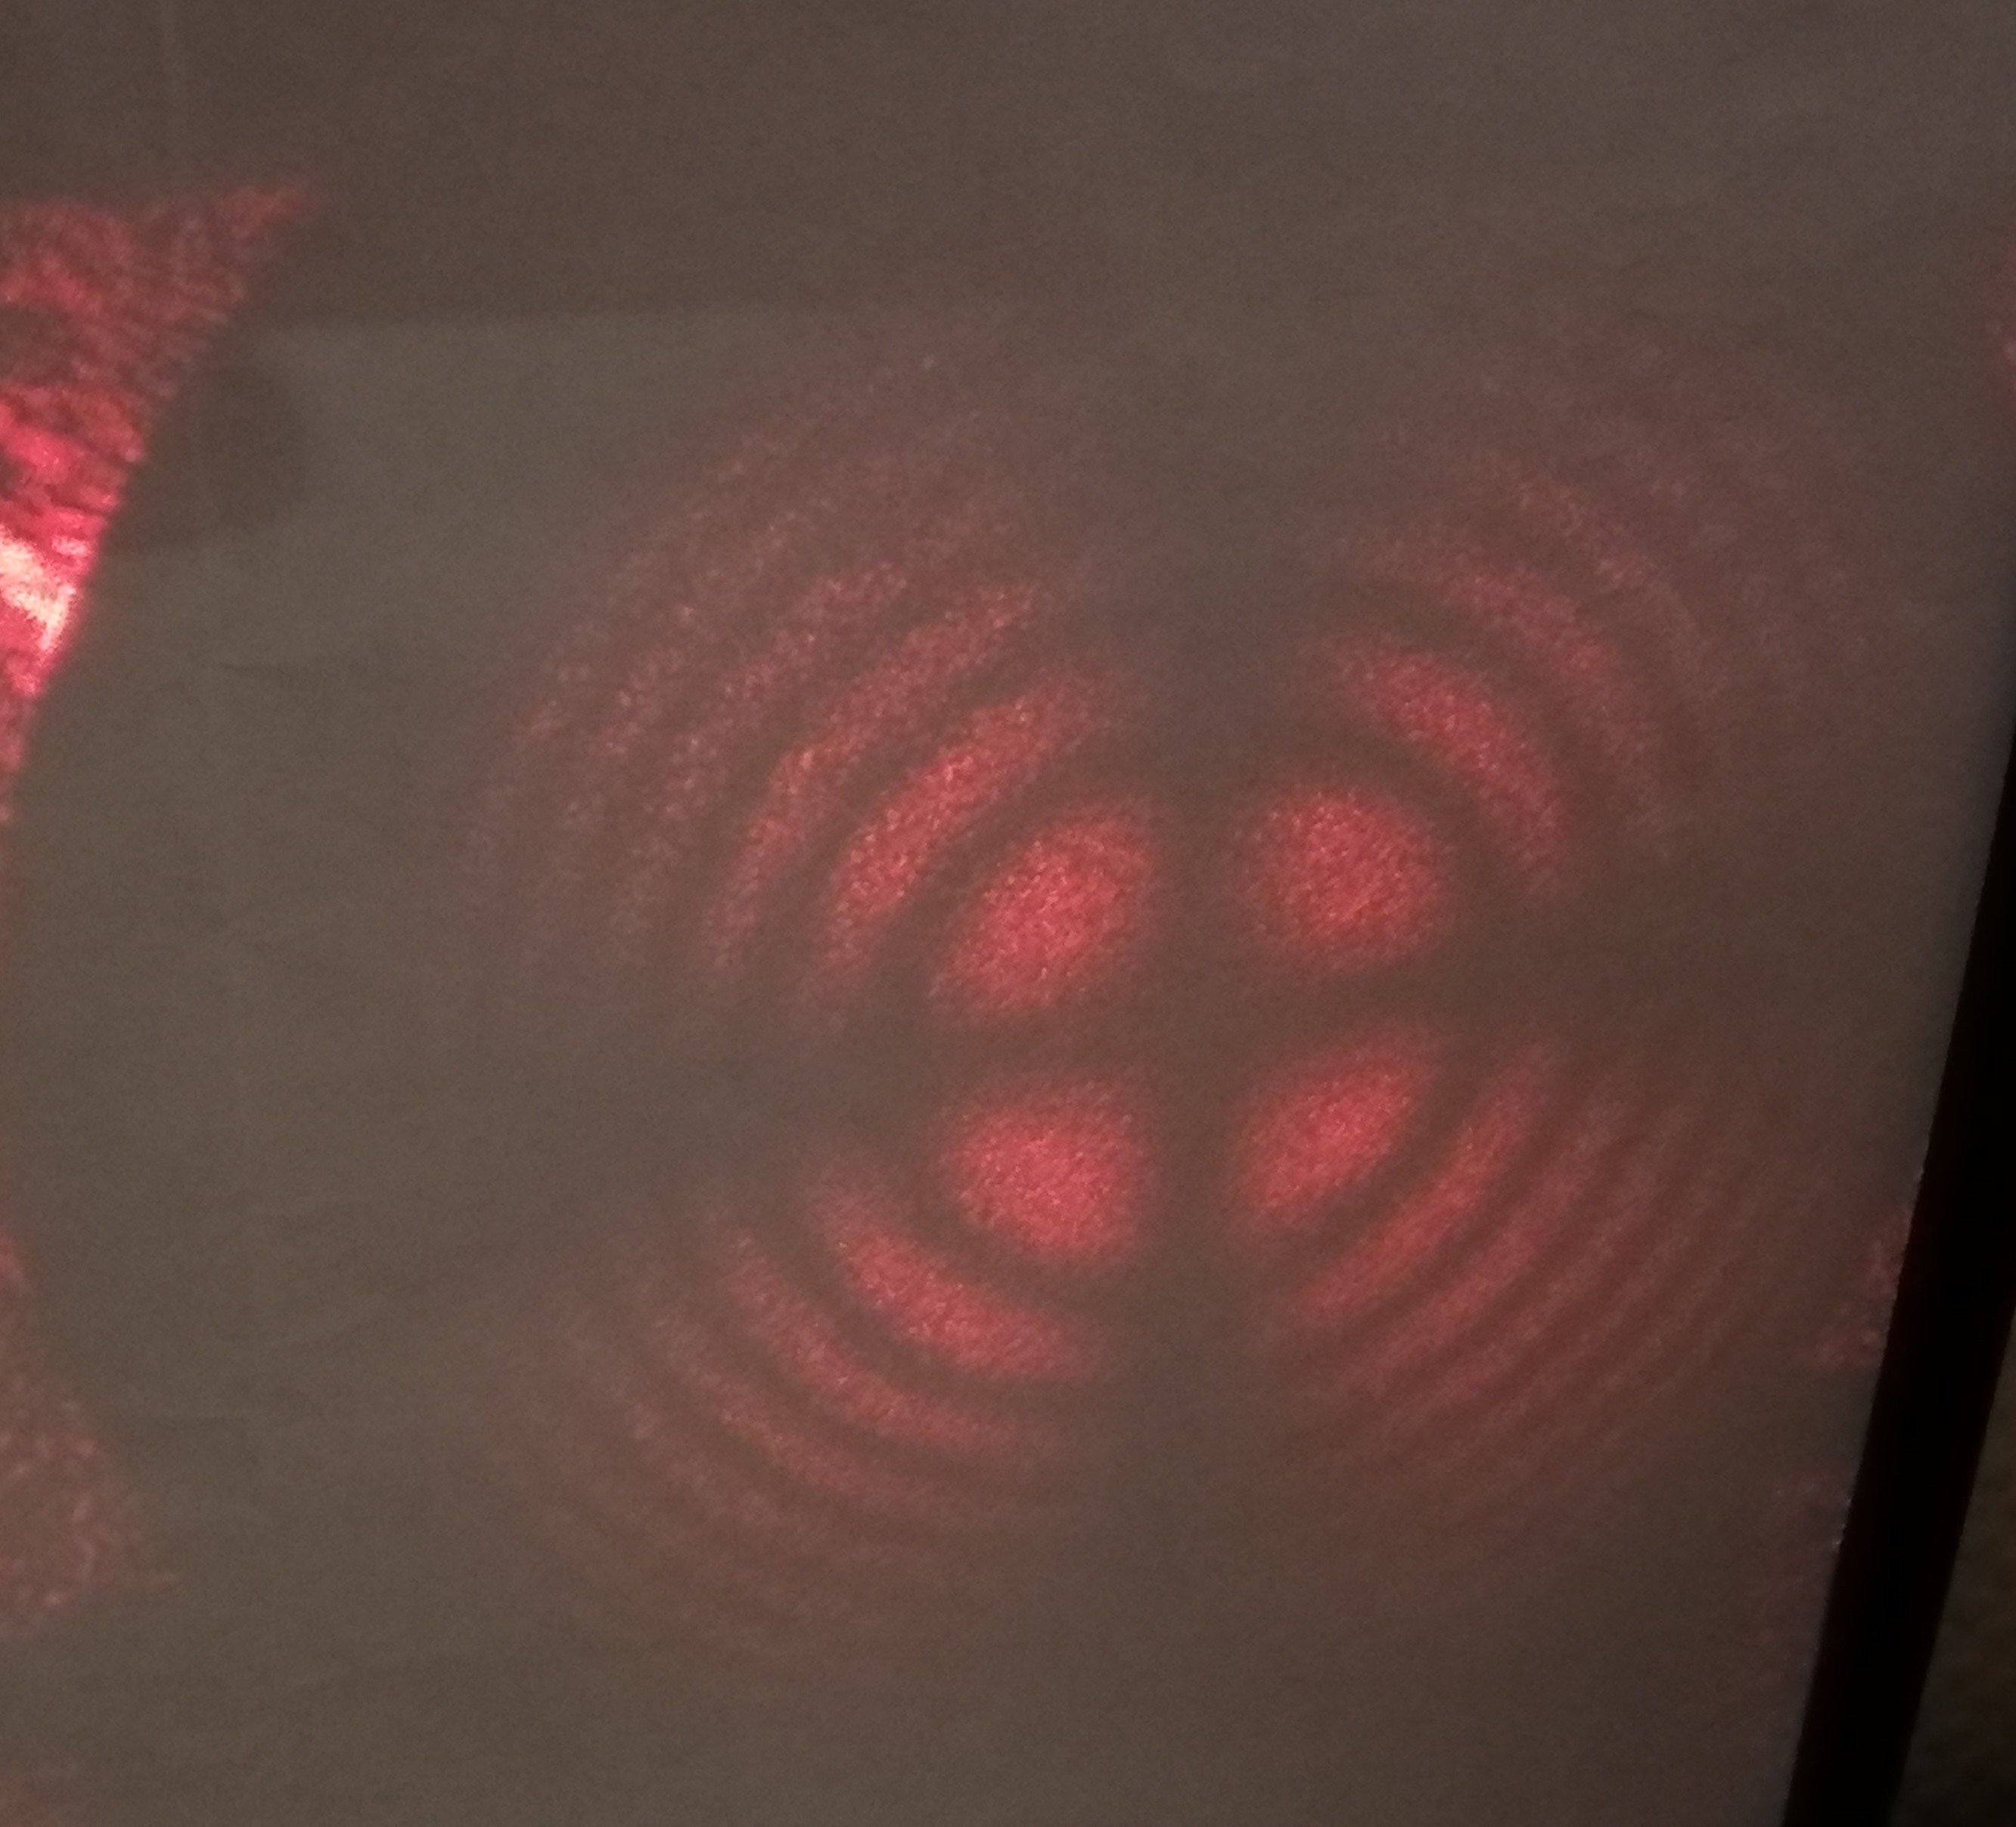
\includegraphics[height=3.5cm]{res/interf3.jpg}
					\vspace{-10pt}
					\caption{\footnotesize  Interference pattern}
					\vspace{-20pt}
				\end{figure}
				\begin{figure}
					\centering
					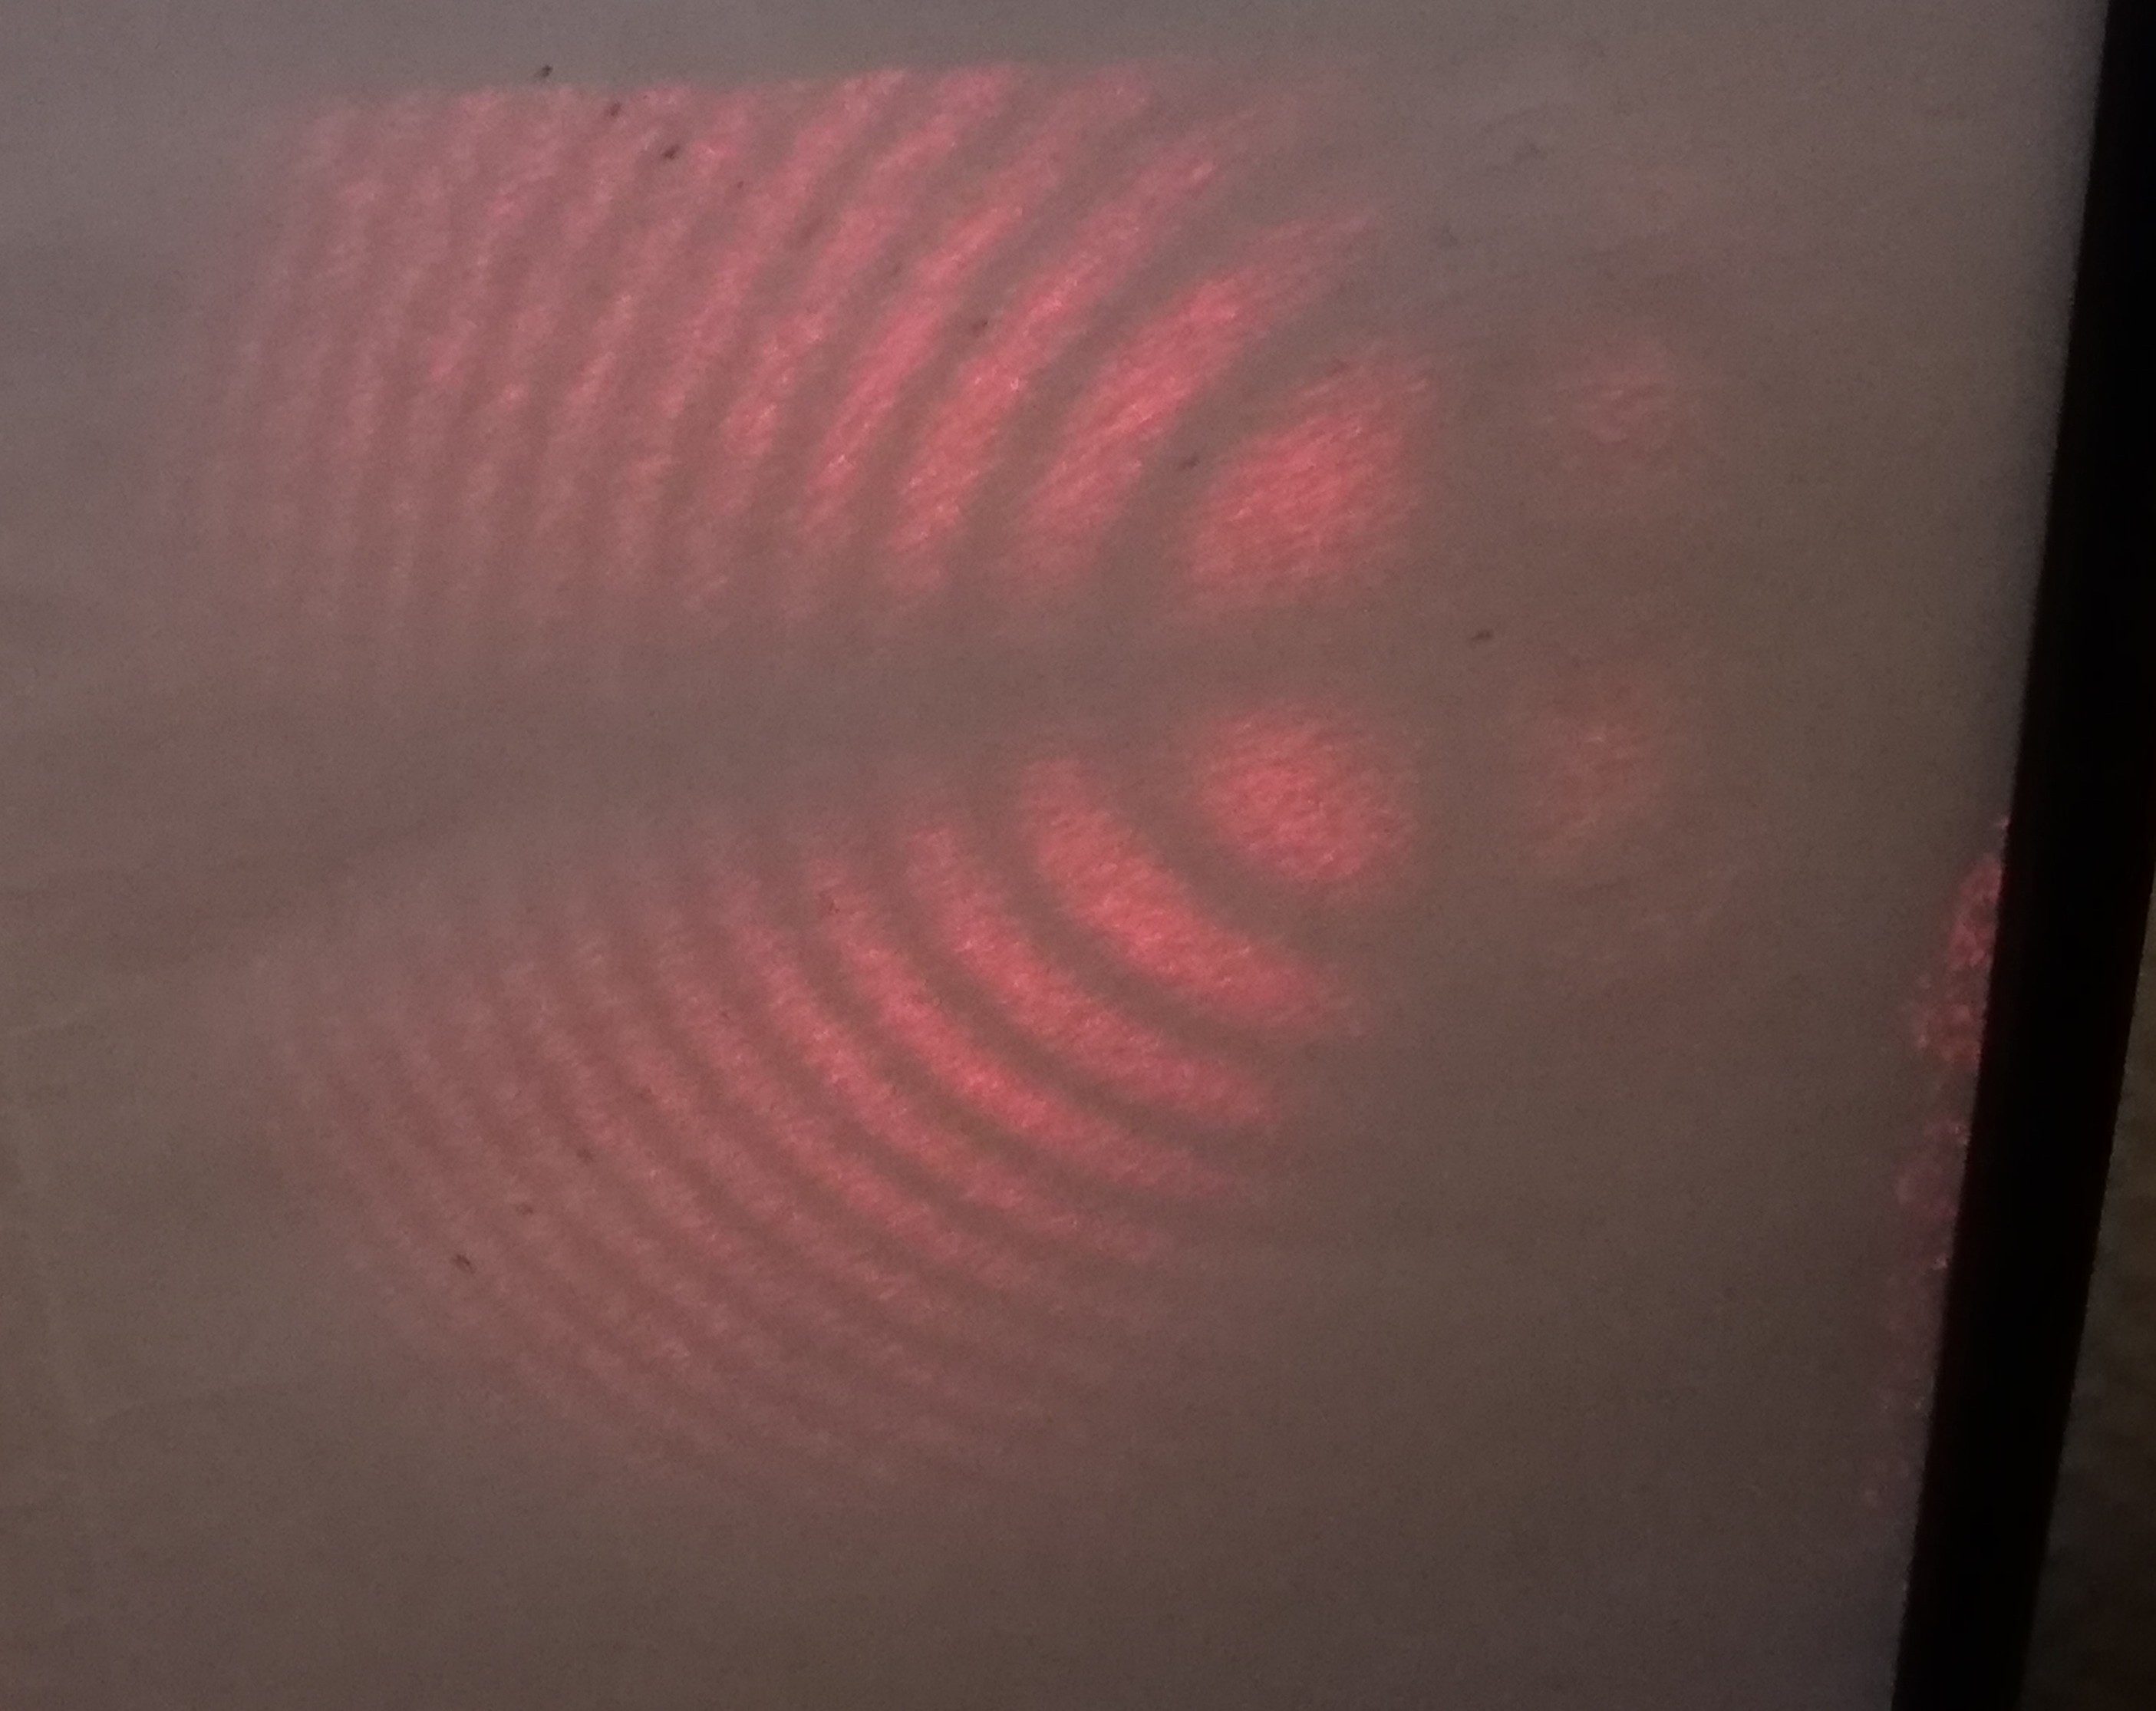
\includegraphics[height=3.5cm]{res/additional_lines.jpg}
					\vspace{-10pt}
					\caption{\footnotesize  Additional lines}
					\vspace{-15pt}
				\end{figure}
			\end{column}
			\begin{column}{0.5\textwidth}
				\begin{figure}
					\vspace{-20pt}
					
					\centering
					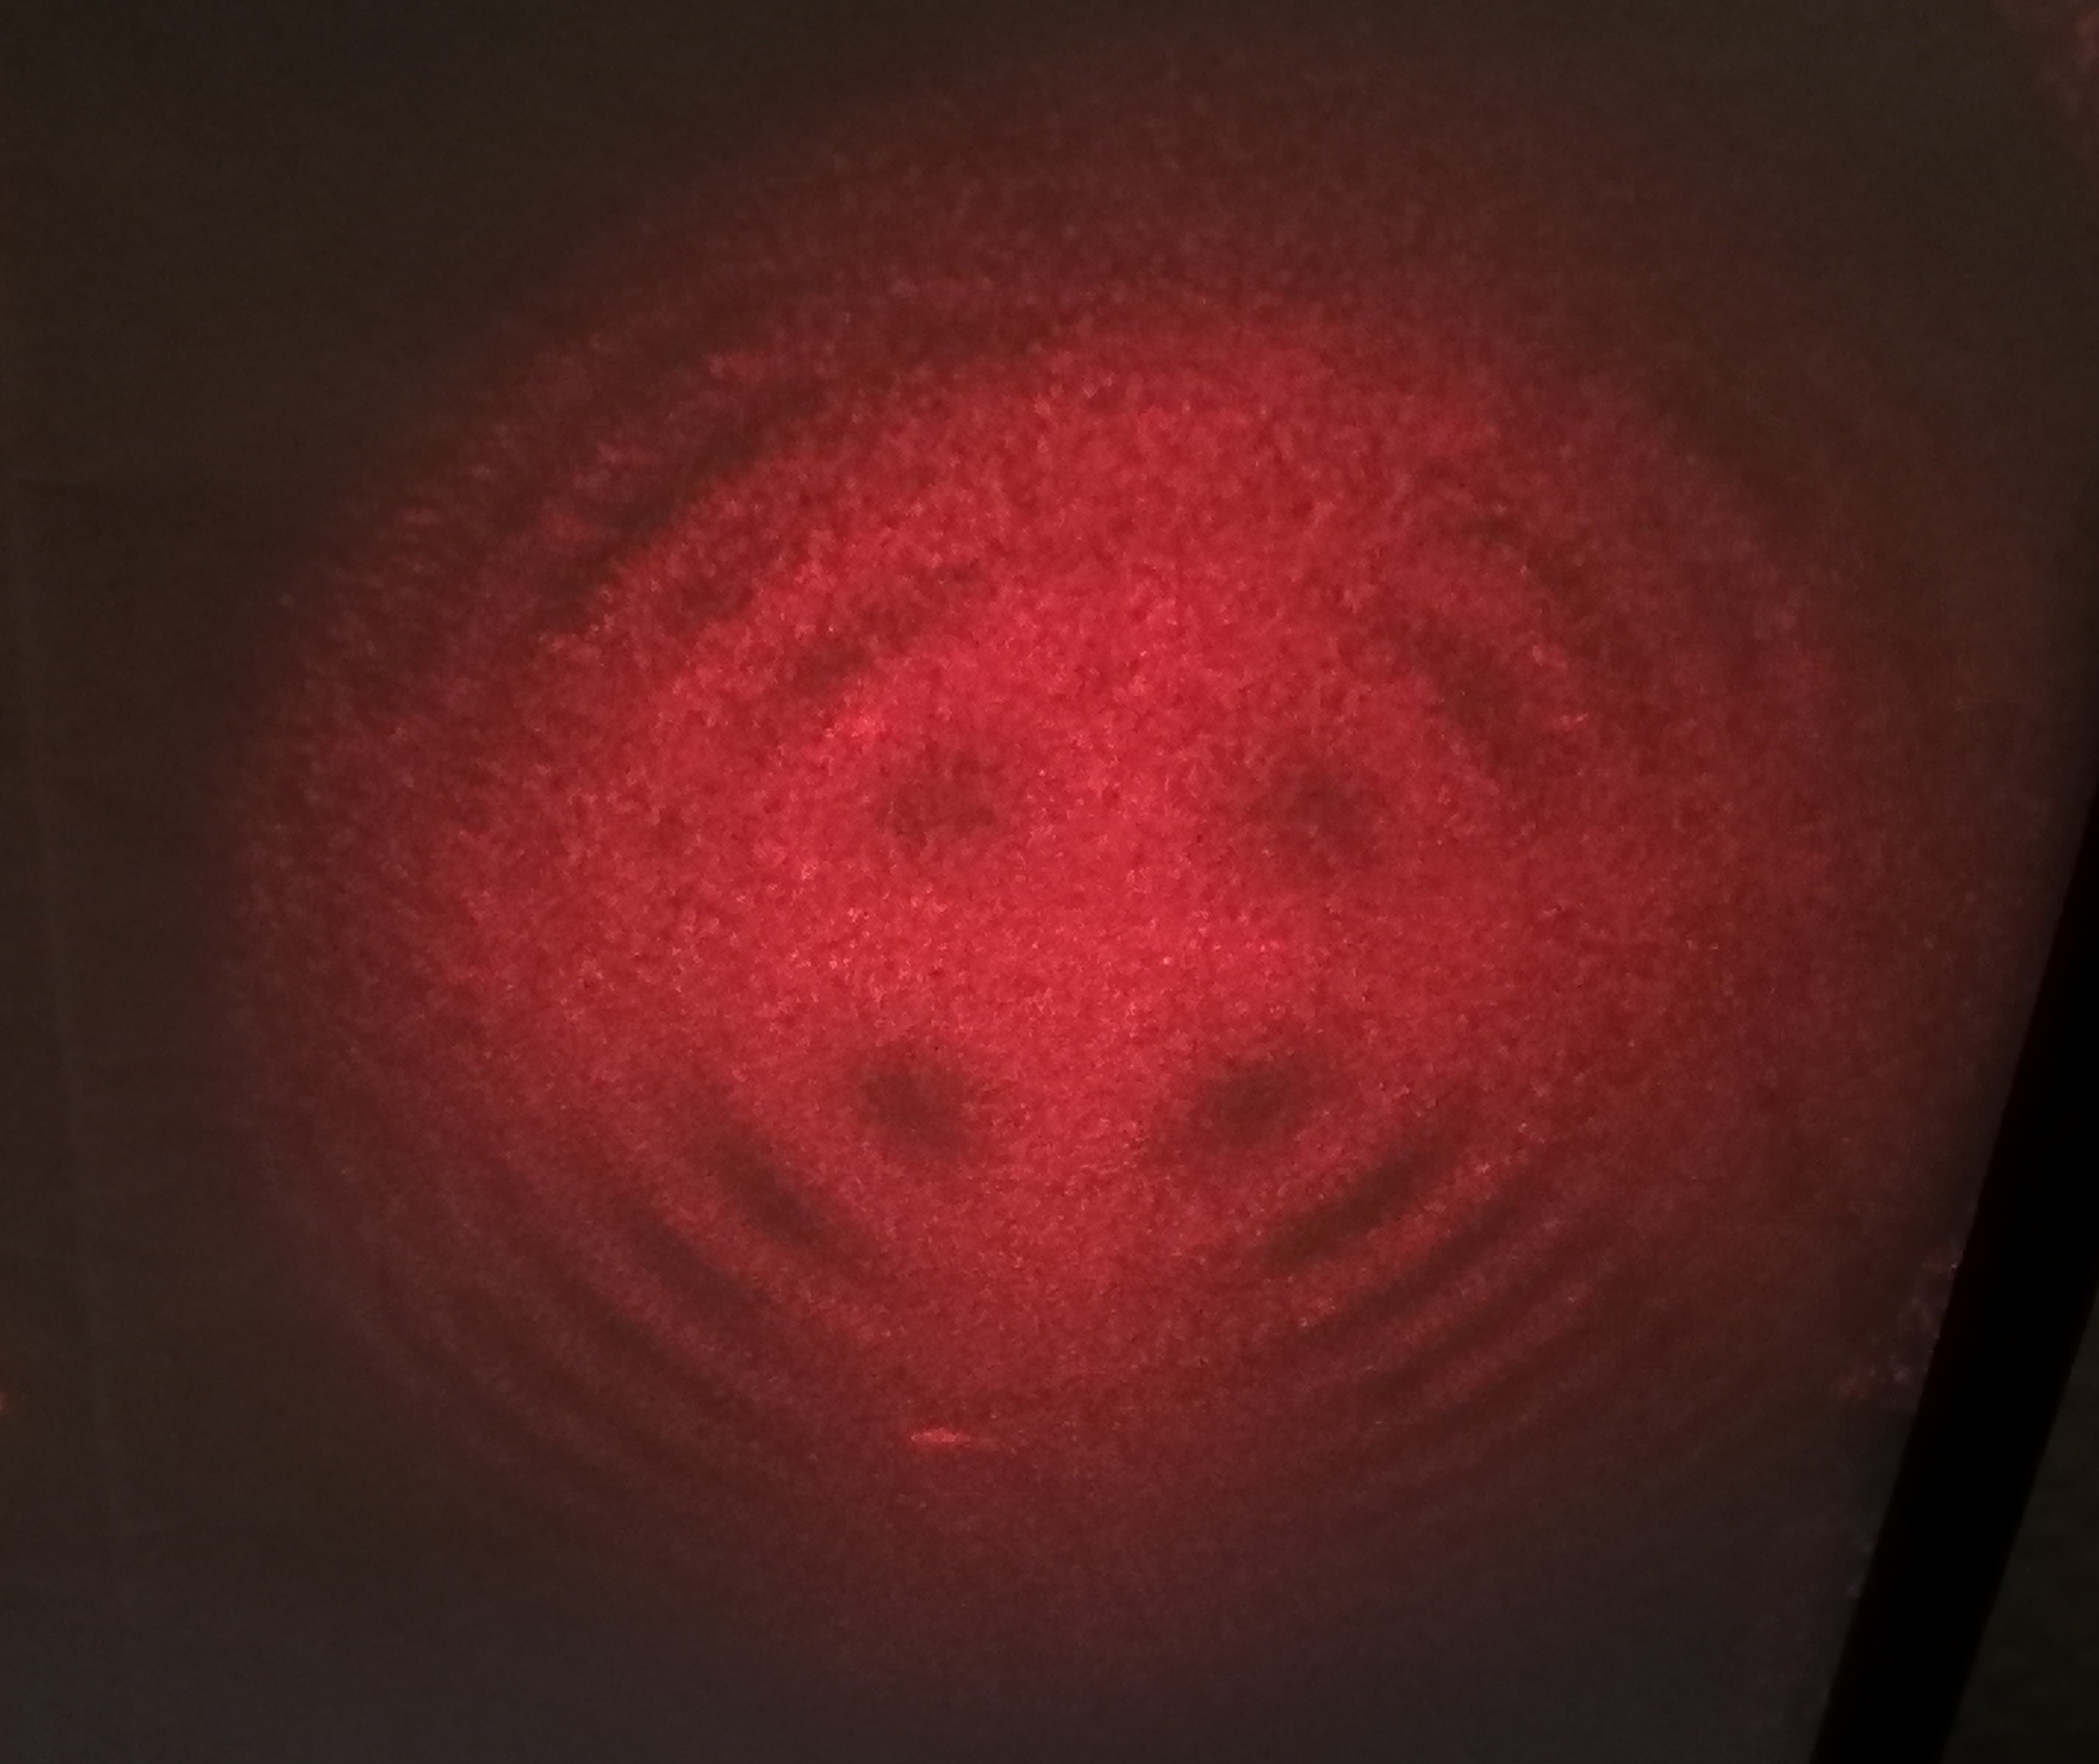
\includegraphics[height=3.5cm]{res/interf_inv2.jpg}
					\vspace{-10pt}
					\caption{\footnotesize  Inverted interference pattern}
					\vspace{-10pt}
				\end{figure}
			
				"Dark circles" conoscopic pattern with "maltese cross".
			
				Rotating polarizer by $90^{\circ}$ we obtain inverted pattern.
				
				Moving polarizer in cross-axis provides more lines to observe.
			\end{column}
		\end{columns}	
	
	\end{frame}

	\begin{frame}
		\frametitle{Dark circles}
		
		\begin{figure}
			\centering
			\includegraphics[width=0.8\linewidth]{gen/r2m.pdf}
			\vspace{-10pt}
			\caption{\footnotesize  Inverted interference pattern}
		\end{figure}
	
		Using slope coefficient and formula for circles' radius we get:
		$$ n_0 - n_e = 0.115 \pm 0.005.$$
	
	\end{frame}	
	
	\begin{frame}
		\frametitle{Pockels Effect}
		
		\begin{columns}
			\begin{column}{0.5\textwidth}
				\begin{figure}
					\centering
					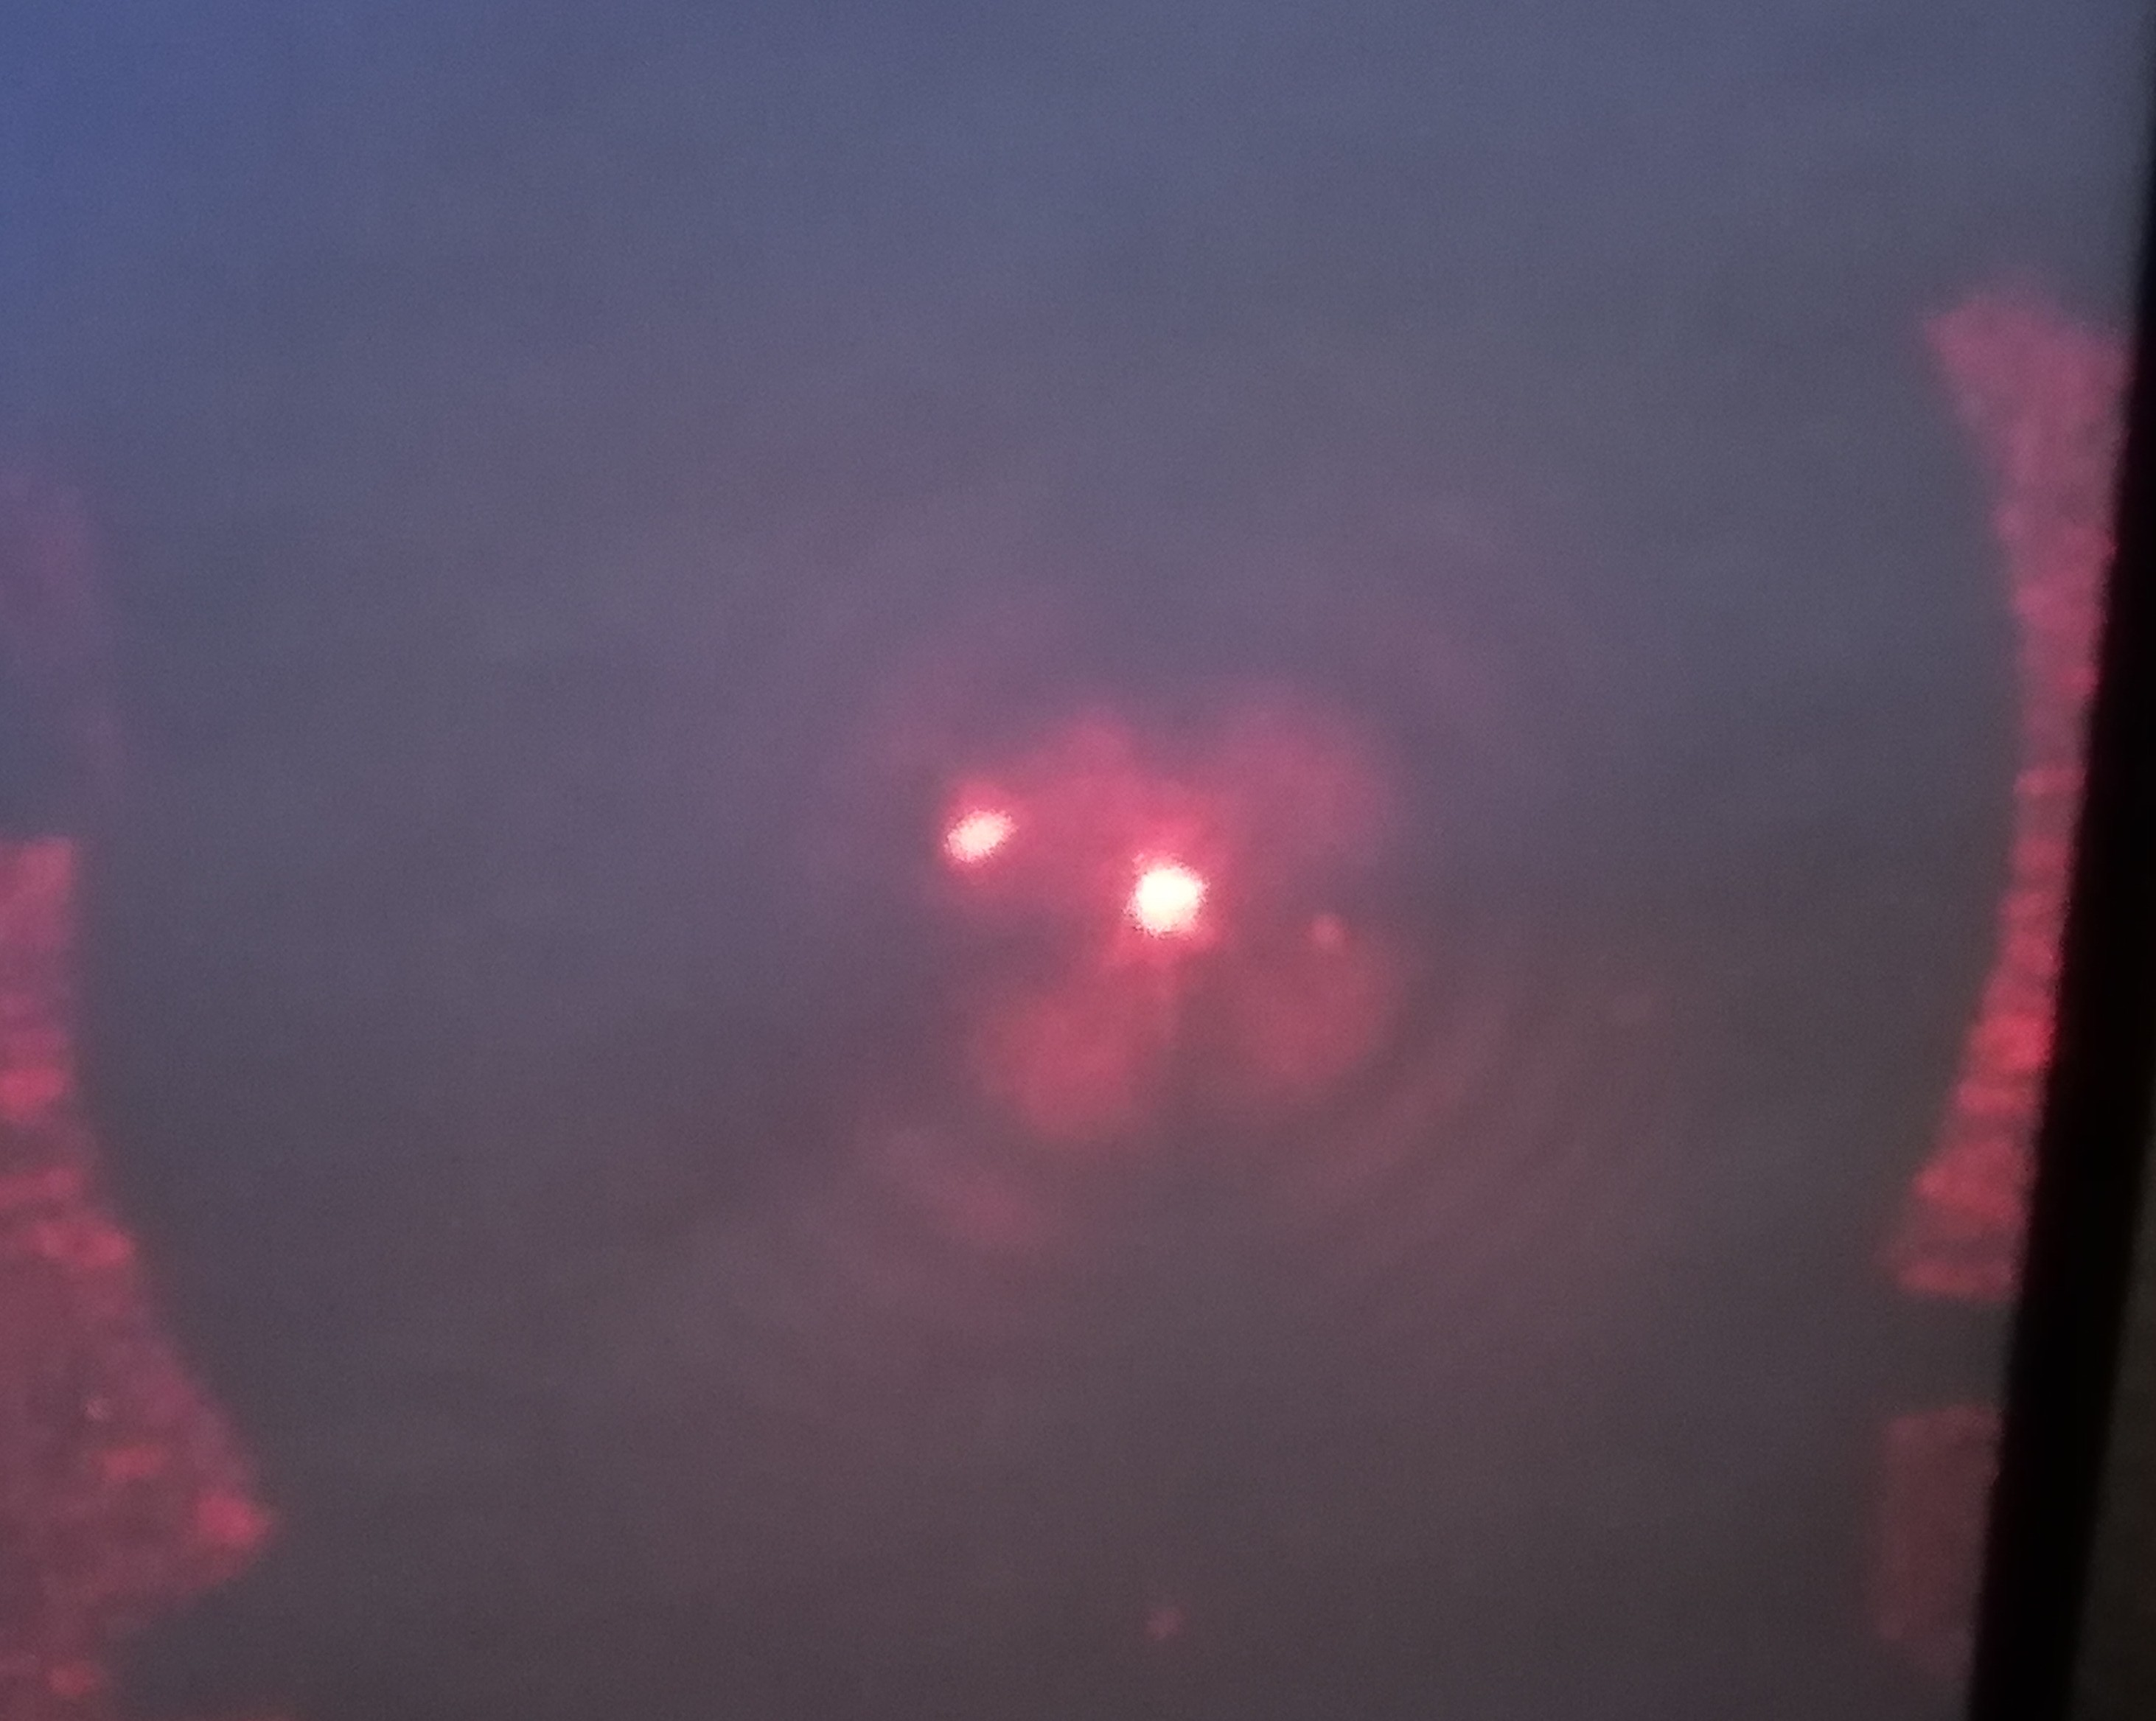
\includegraphics[height=3.5cm]{res/u_0.jpg}
					\vspace{-10pt}
					\caption{\footnotesize  $U = 0$}
				\end{figure}
			
			\end{column}
			\begin{column}{0.5\textwidth}
				\begin{figure}
					\centering
					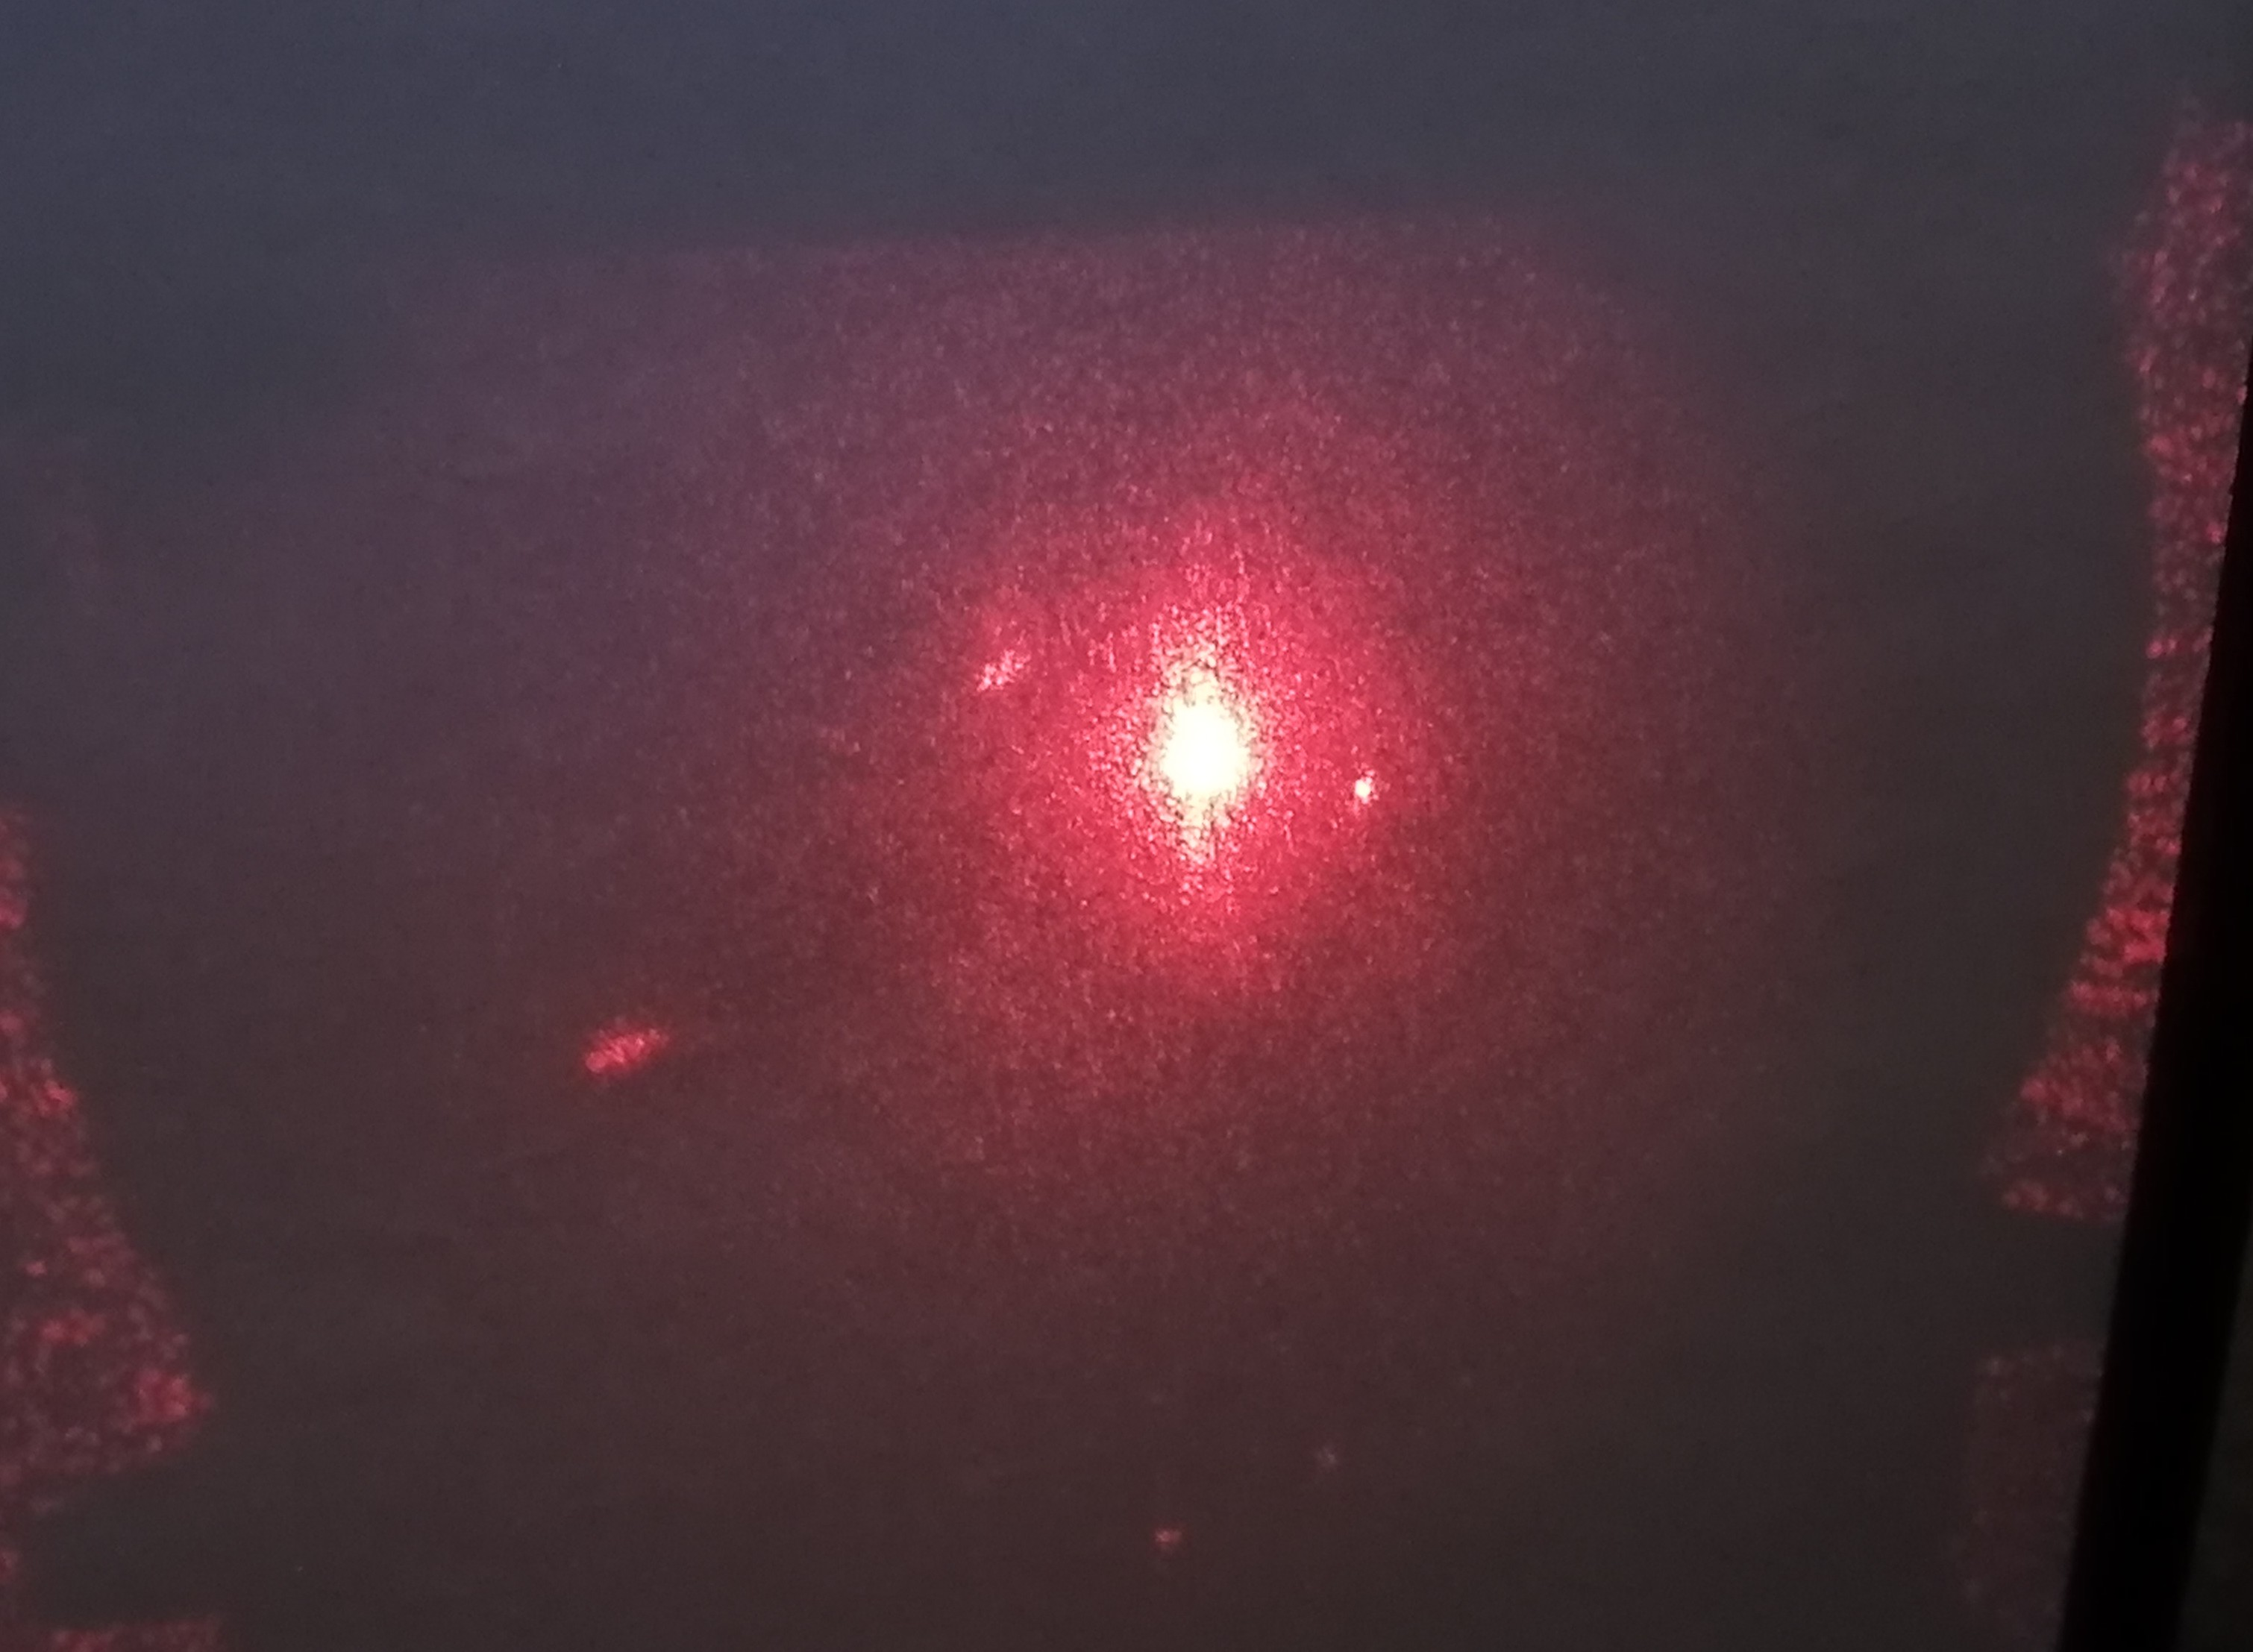
\includegraphics[height=3.5cm]{res/u_l_2.jpg}
					\vspace{-10pt}
					\caption{\footnotesize  $U = U_{\lambda/2}$}
				\end{figure}
			\end{column}
		\end{columns}
	
		\begin{columns}
			\begin{column}{0.4\textwidth}
				\begin{table}[]
					\begin{tabular}{lll}
						\hline
						& \multicolumn{2}{l}{$U, \text{kV}$} \\
						m & $\perp$    & $\parallel$    \\ \hline
						1 & 0.45         & 0.45             \\
						2 & 0.90         & 0.87             \\
						3 & 1.38         & 1.35             \\ \hline
					\end{tabular}
				\end{table}
			\end{column}
		
			\begin{column}{0.6\textwidth}
				Applying voltage on $\text{LiNbO}_3$ crystal we observe Pockels effect.
				
				Measuring voltages we get:
				$$U_{\lambda/2} = (0.45 \pm 0.03)\; \text{kV}.$$
			\end{column}
		\end{columns}

	\end{frame}

	\begin{frame}
		\frametitle{Circular Polarization}
		\begin{figure}
			\centering
			\movie[width=\linewidth, height=0.5625\linewidth, poster]{}{res/u_l_4.mp4}
			\caption{Brightness invariance of circularly-polarised light}
		\end{figure}
	\end{frame}

	\begin{frame}
		\frametitle{Lissajous figures}


		\begin{figure}
			\centering
			\includegraphics[width=\linewidth]{res/lissajous.png}
			\vspace{-10pt}
			\caption{\footnotesize  Lissajous figures for $\parallel$ (top) and $\perp$ (bottom) polarizations}.
		\end{figure}
				
	\end{frame}

	\begin{frame}
		\frametitle{Lissajous figures transformation}
		\begin{figure}
			\centering
			\movie[width=\linewidth, height=0.5625\linewidth, poster]{}{res/rotation.mp4}
			\caption{Effect of polarizer rotation on lissajous figures}
		\end{figure}
				
		
	\end{frame}

	\begin{frame}
		\frametitle{Conclusion}
		
		Birefrigence was observed. Difference of refractive indices for ordinary and extraordinary waves (LiNbO$_3$ -- 'negative' crystal):
		$$ n_e - n_o = -(0.115 \pm 0.005).$$
		Reference value (for $\lambda = 630 \; \text{nm}$, depends on crystal composition)\footnote{\href{https://doi.org/10.1063/1.352951}{
			Refractive indices of lithium niobate as a function of wavelength and composition 
			Journal of Applied Physics 73, 3472 (1993)}}
		:
		$$ n_e - n_o = 0.07 \div 0.12.$$
		
		Pockels effect was examined. $U_{\lambda/2}$ was measured:
		$$ U_{\lambda/2} = (0.45 \pm 0.03) \; \text{kV}\quad \Rightarrow \quad E_{\lambda/2} = (150 \pm 9) \; \text{kV}/\text{m}.$$
	\end{frame}
	
	\begin{frame}[plain,c]
		\begin{center}
			\huge \usebeamercolor[fg]{frametitle} Thank you for your attention!
		\end{center}
	\end{frame}
		
	
\end{document}